\documentclass{article}
\usepackage{iclr2026_conference,times}
\input{math_commands.tex}

\usepackage{hyperref}
\usepackage{url}
\usepackage{graphicx}
\usepackage{booktabs}
\usepackage{amsmath}
\usepackage{xcolor}
\usepackage{array}

\graphicspath{{figures/}}

\title{Frozen Protein Language Models Encode Viral\\
Evolutionary Geometry Across Two Scales}

\author{%
  James Huang \\
  Department of Computer Science \& Engineering \\
  University of Minnesota, Twin Cities \\
  Minneapolis, MN 55455 \\
  \texttt{huan1786@umn.edu}
}

\newcommand{\fix}{\marginpar{FIX}}
\newcommand{\new}{\marginpar{NEW}}

\iclrfinalcopy  % display author names per instructor requirement

\begin{document}

\maketitle

\begin{abstract}
We ask whether a protein language model trained on masked residue prediction---with no evolutionary labels of any kind---encodes viral taxonomy and within-species variant structure simultaneously. Using frozen ESM-2 embeddings, we build two systems sharing the same backbone: a supervised four-rank cascade decoder (Kingdom $\to$ Phylum $\to$ Class $\to$ Order) for cross-species taxonomy, and an unsupervised SVD-HDBSCAN pipeline for intra-species variant surveillance. The supervised system reaches 90.57\% top-1 Order accuracy with 94.86\% hierarchical consistency. For surveillance, ESM-2 mutation-identity representations explain variance in SARS-CoV-2 Spike sequences 280$\times$ better than Hamming distance does, and unsupervised clustering achieves silhouette $= 0.895$, ARI $= 0.992$---without alignment or any lineage labels. Among predicted noise points, BA.2/5+ sequences show a 52.3\% noise rate driven by mosaic recombination signatures. Taken together, these results indicate that evolutionary geometry is a structural property of ESM-2's representation space, not an artifact of downstream fine-tuning.
\end{abstract}

% ──────────────────────────────────────────────────────────────────────────────
\section{What Problem}
\label{sec:problem}
% ──────────────────────────────────────────────────────────────────────────────

Viral surveillance operates at two very different scales. At the \textit{cross-species} scale, taxonomists assign newly discovered viruses to kingdoms, phyla, classes, and orders using the ICTV hierarchy. At the \textit{intra-species} scale, epidemiologists track variants of concern (VOCs) within a single species---SARS-CoV-2 lineages being the clearest recent example. Both problems have traditionally relied on sequence alignment: multiple sequence alignment (MSA) for phylogenetics, and reference-aligned Pango lineage calls for VOC monitoring.

Alignment-based approaches carry practical costs. MSA is $O(n^2)$ in sequence length, breaks on highly divergent sequences, and cannot handle insertion/deletion-rich regions without manual curation. Pango lineage calls require expert-maintained rules and break down at recombinant junctions---the BA.2/5+ designation, for instance, lumps sequences from at least three distinct recombinant histories.

Deep learning offers a different path. ESM-2 \citep{lin2023esm2}, trained via masked residue prediction on UniRef, produces dense 320--1280-dimensional representations that have been shown to encode secondary structure, residue contacts, and thermostability---none of which appear in the training objective explicitly. We ask a sharper version of this question: do frozen ESM-2 embeddings encode evolutionary signals useful for both cross-species taxonomy and intra-species variant monitoring, using the same backbone and no alignment?

This project works at that intersection. The two-system architecture is not primarily an engineering convenience; it is the experimental design that lets us test whether the observed signals are intrinsic to ESM-2's representation space or artifacts of task-specific training.

% ──────────────────────────────────────────────────────────────────────────────
\section{Why Interesting}
\label{sec:interesting}
% ──────────────────────────────────────────────────────────────────────────────

\textbf{ESM-2 never saw a taxonomy label.} It was trained to predict masked amino acids. If its frozen representations simultaneously support four-rank ICTV classification and single-residue VOC detection, that is evidence of implicit evolutionary geometry, not task-specific memorization. The analogy is word2vec encoding syntactic structure without any part-of-speech supervision.

\textbf{Two scales, one backbone.} The cross-species task uses ESM-2-8M (6 layers, 320-d); the surveillance task uses ESM-2-650M (33 layers, 1280-d). Both are frozen. The fact that the same family of representations works at both the Kingdom/Order level and the single-amino-acid-substitution level suggests the geometry is multi-resolution, not scale-specific.

\textbf{Euclidean distance fails; local topology survives.} A key finding is that global Euclidean distance in ESM-2 space poorly predicts lineage membership, yet local $k$-NN topology is stable and biologically meaningful. This places ESM-2 representations on a curved manifold---alignment-based methods flatten that manifold artificially; density-based methods can work with it directly.

% ──────────────────────────────────────────────────────────────────────────────
\section{Previous Work}
\label{sec:related}
% ──────────────────────────────────────────────────────────────────────────────

\textbf{Protein language models.} \citet{rives2021esm} showed that ESM-1b representations encode structural and evolutionary information without explicit supervision. \citet{lin2023esm2} scaled this to ESM-2 (8M--15B parameters) with improved masked language model training on UniRef90/UniRef50. Downstream probing studies have demonstrated that these representations carry contact maps, secondary structure, and stability predictions.

\textbf{Viral taxonomy with deep learning.} \citet{deng2024numerical} proposed numerical taxonomy enabled by bio-language models, providing the architectural reference for our cascade decoder design. \citet{passion2025virusproject} released an ESM-based pipeline that translates viral RNA in three frames, embeds with ESM-2, and feeds a multi-task head for class/order classification. Our work extends that pipeline to a full four-rank hierarchy with a tandem cascade decoder and an autoregressive output head trained with a layer-affiliate hierarchical loss.

\textbf{Unsupervised variant monitoring.} Alignment-free methods for VOC clustering include $k$-mer representations \citep{wood2019kraken2} and co-occurrence matrix decompositions. Reference-aligned approaches (Pango, Nextclade) dominate in practice but require continuous expert curation. HDBSCAN \citep{mcinnes2017hdbscan} provides density-based clustering without a preset $k$, making it appropriate for an evolving variant landscape. We combine it with truncated SVD to remove nuisance dimensions in ESM-2 space.


% ──────────────────────────────────────────────────────────────────────────────
\section{Goals}
\label{sec:goals}
% ──────────────────────────────────────────────────────────────────────────────

We organize the work around three testable hypotheses.

\textbf{H1} (cross-species): Frozen ESM-2 + cascade decoder $\geq 90\%$ top-1 Order accuracy, $\geq 94\%$ hierarchical consistency.
\textbf{H2} (clustering): SVD-HDBSCAN silhouette $\geq 0.7$, ARI $\geq 0.9$ on SARS-CoV-2 without lineage labels; noise points enrich known recombinants.
\textbf{H3} (mechanism): (a) mutation-identity R$^2 \gg$ Hamming R$^2$ across $\geq 3$ virus families; (b) lineage signal present in Layer 1; (c) top IG residues fall inside known functional domains.

% ──────────────────────────────────────────────────────────────────────────────
\section{Methods}
\label{sec:methods}
% ──────────────────────────────────────────────────────────────────────────────

\subsection{Cross-species taxonomy (supervised)}

Figure~\ref{fig:pipeline-sup} summarizes the three-stage supervised pipeline (frozen embedding $\to$ genome aggregation $\to$ cascade decoding). We describe each component below; Figure~\ref{fig:arch} tabulates the design choice and rationale for every block.

\begin{figure}[!htbp]
  \centering
  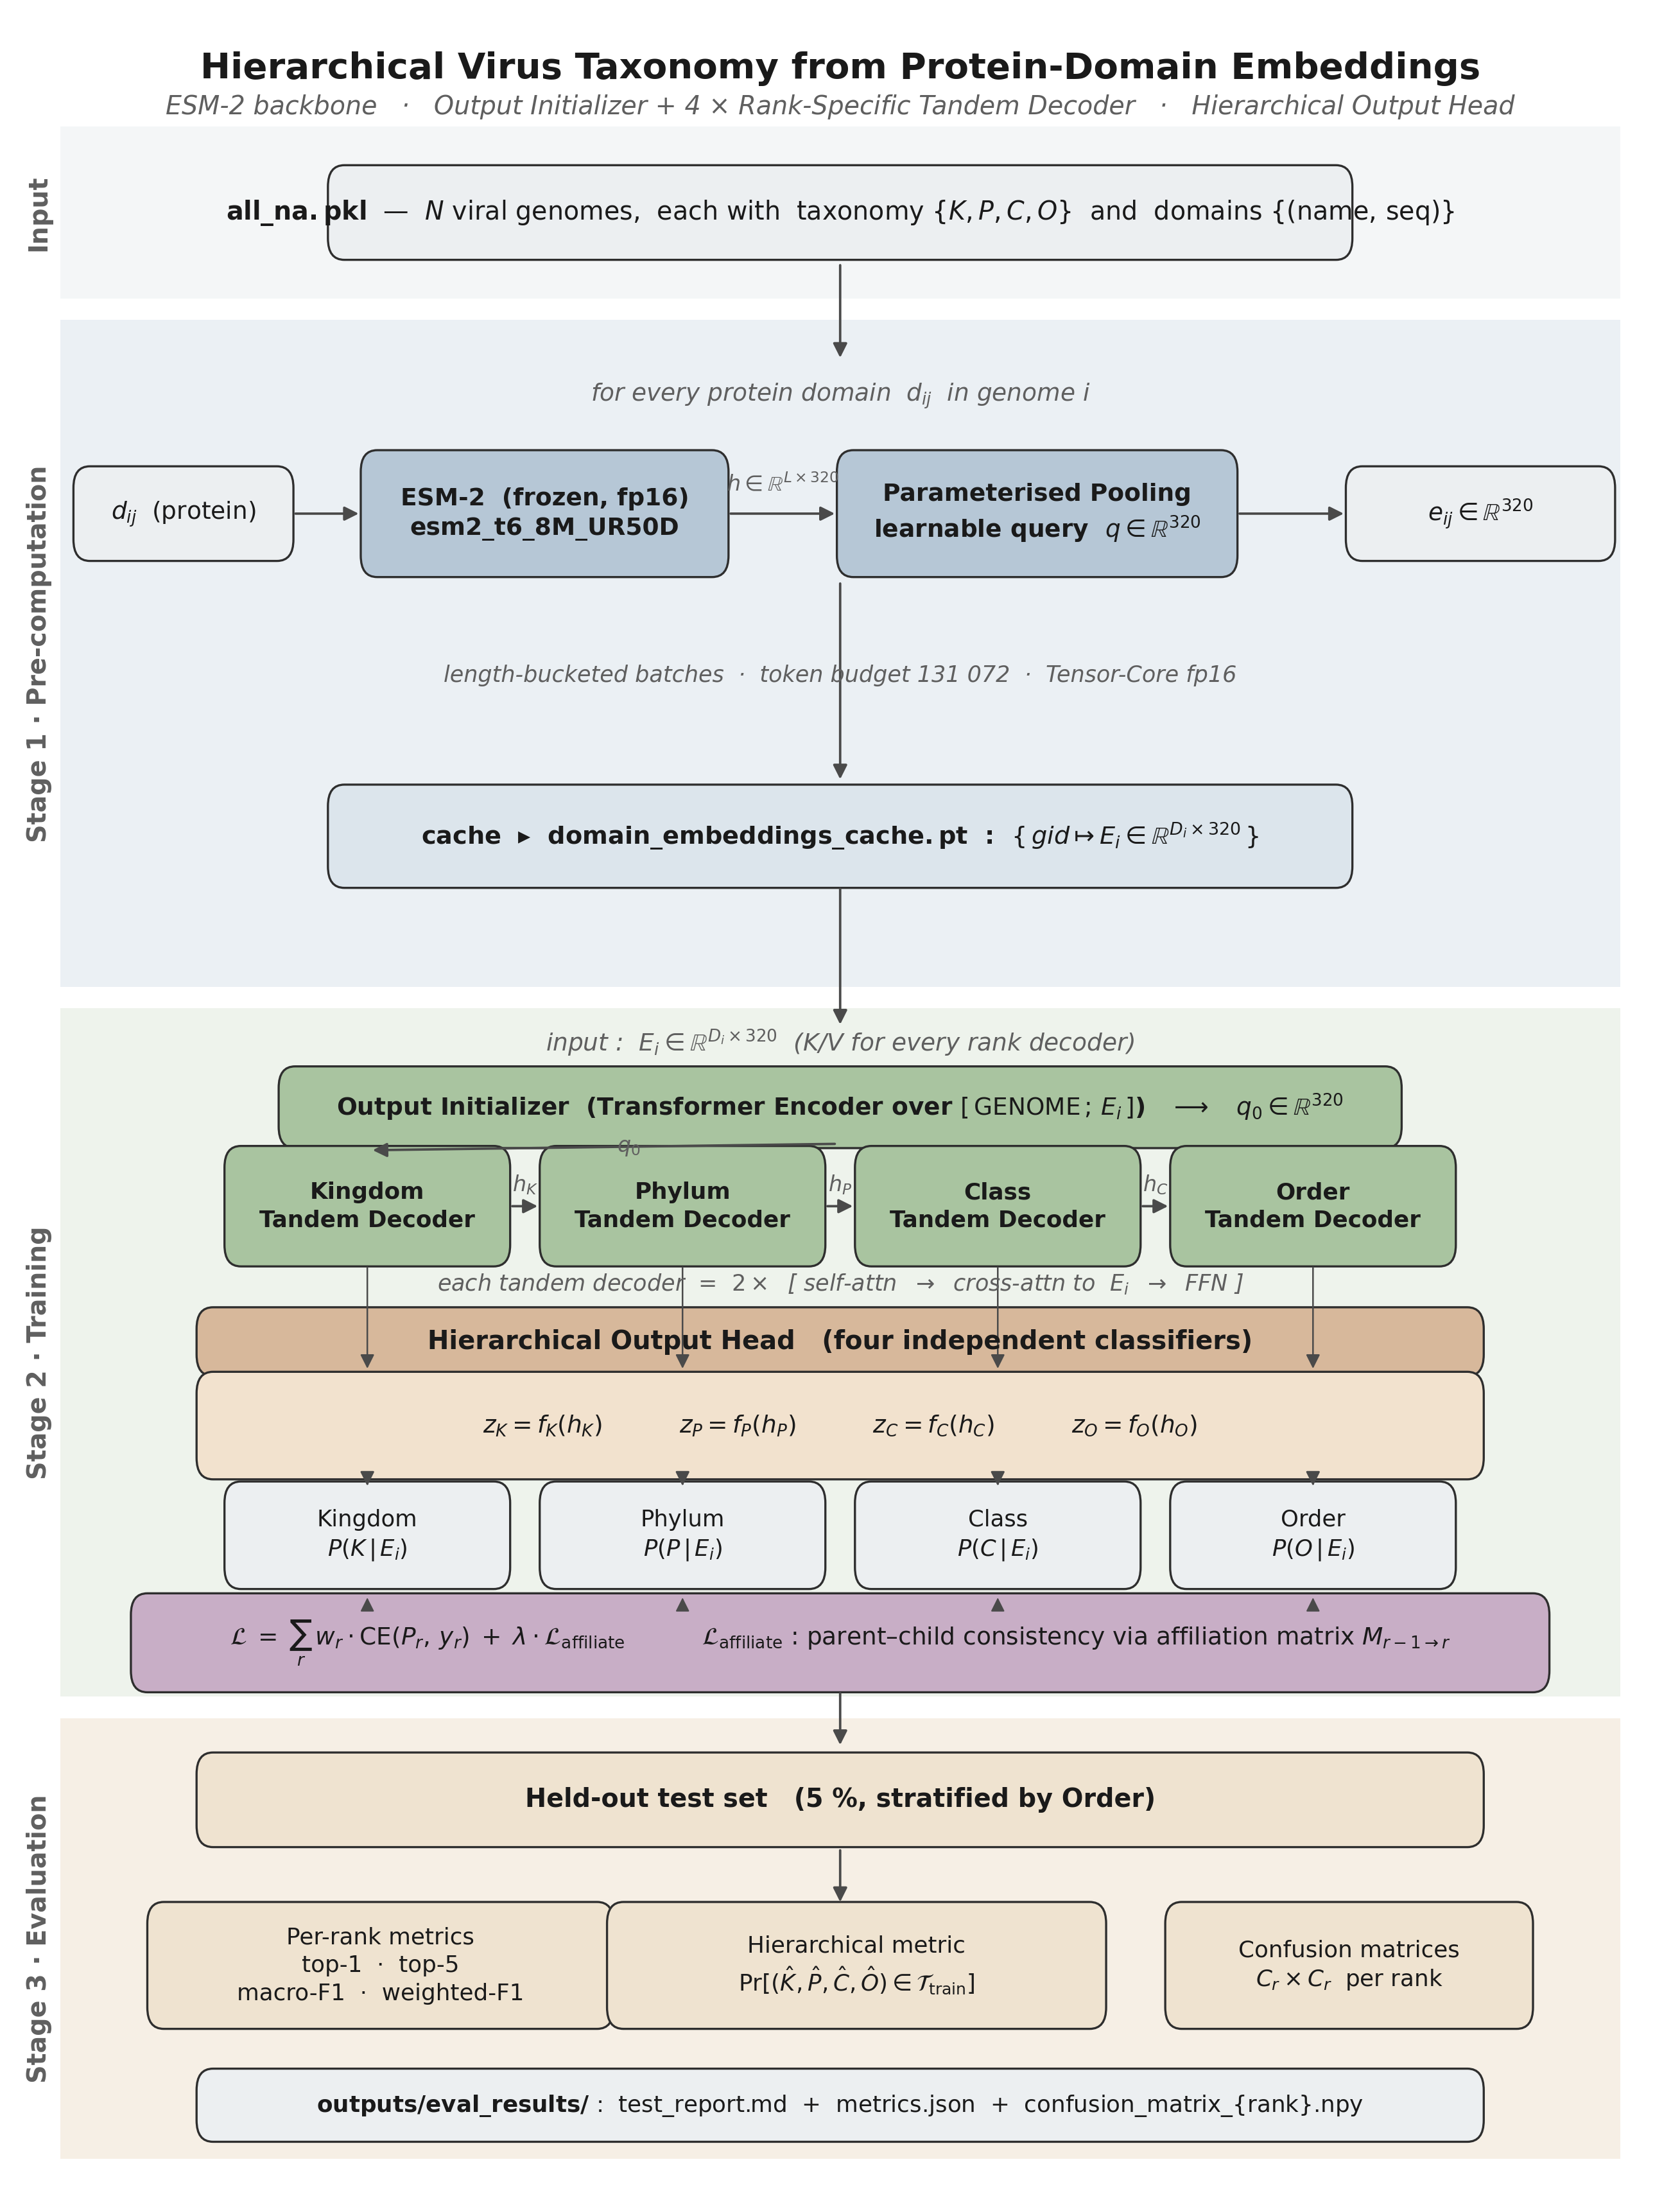
\includegraphics[width=\linewidth]{fig_pipeline_supervised.png}
  \caption{Supervised pipeline (three stages). \textbf{Stage 1:} frozen ESM-2-8M embeds each Pfam domain; a parameterized attention pooling with learnable query $\mathbf{q}\!\in\!\mathbb{R}^{320}$ produces one 320-d vector per domain. \textbf{Stage 2:} an OutputInitializer (2-layer Transformer encoder over genome) aggregates all domain vectors into a genome context $g\!\in\!\mathbb{R}^{320}$. \textbf{Stage 3:} four tandem cascade decoders produce rank-specific embeddings autoregressively (K$\!\to\!$P$\!\to\!$C$\!\to\!$O); the affiliate loss enforces parent-child consistency via the ICTV affinity matrix $\mathbf{M}$.}
  \label{fig:pipeline-sup}
\end{figure}

\textbf{Data.} Viral genomes with ICTV four-rank labels \citep{passion2025virusproject}, split 80/15/5 by Order-stratified sampling. Pfam domains via 6-frame translation; pre-computed embeddings cached at token budget 131{,}072.

\textbf{Domain encoder.} Frozen ESM-2-8M (6 layers, 320-d). A learnable query $\mathbf{q} \in \mathbb{R}^{320}$ attends over per-token ESM-2 outputs (parameterized attention pooling), producing one 320-d vector per domain. Pre-computing embeddings once drops training from $\sim$7 s/step to $\sim$50 ms/step.

\textbf{Cascade decoder and loss.} Figure~\ref{fig:arch} diagrams the autoregressive architecture. Each of the four tandem decoders runs: $[\text{self-attn} \to \text{cross-attn}(E) \to \text{FFN}] \times 2$, with rank $r$'s output serving as a conditioning prefix for rank $r{+}1$. The joint loss is:
\[
  \mathcal{L} = \textstyle\sum_{r} w_r \,\mathrm{CE}(p_r, y_r) \;+\; \lambda \sum_r \bigl\|\mathrm{softmax}(\hat{p}_r) - \mathbf{M}_{r-1,r}\,\mathrm{softmax}(\hat{p}_{r-1})\bigr\|_1
\]
$\mathbf{M}_{r-1,r}$ is the ICTV parent-child affinity matrix; the second term is the \emph{affiliate loss}, penalizing rank-inconsistent predictions.

% ── Architecture table: cascade decoder design ──────────────────────────────
\begin{figure}[!htbp]
\centering
\renewcommand{\arraystretch}{1.1}
\begin{tabular}{>{\bfseries\small}p{0.22\linewidth}
                >{\small}p{0.41\linewidth}
                >{\small\itshape}p{0.28\linewidth}}
\toprule
\textbf{Component} & \textbf{Design} & \textbf{Why} \\
\midrule
ESM-2-8M (frozen) &
  6-layer PLM, 320-d tokens; pre-computed per-domain cache
  (token budget 131{,}072; 140$\times$ speed-up) &
  Biological priors from 250M proteins; no task labels needed \\

Attention Pooling &
  Single learnable query $\mathbf{q}\!\in\!\mathbb{R}^{320}$ attends over tokens;
  domain $\to$ 320-d vector &
  Data-driven focus on discriminative positions vs.\ uniform mean-pool \\
\midrule
Tandem Decoder $\times$4 &
  One decoder per rank; each runs
  [self-attn $\to$ cross-attn($E$) $\to$ FFN]$\times$2;
  rank-specific learnable query $\mathbf{q}_r$ &
  Each rank reads both ESM-2 tokens (via cross-attn) and
  its own query; $\approx$2.4M trainable params \\

Autoregressive K$\to$P$\to$C$\to$O &
  Rank $r$ prediction concatenated as prefix to decoder $r{+}1$ &
  Hierarchy encoded in the \emph{inference graph},
  not only the loss \\
\midrule
Affiliate Loss &
  $+\,\lambda\|\mathrm{softmax}(\hat{p}_r) -
  \mathbf{M}_{r-1,r}\,\mathrm{softmax}(\hat{p}_{r-1})\|_1$
  where $\mathbf{M}$ is the ICTV parent-child affinity matrix &
  Hierarchical consistency: 0.02\% $\to$ 94.86\%
  (four orders of magnitude) \\
\bottomrule
\end{tabular}
\caption{Cascade decoder design summary. Blue rows: frozen backbone + pooling (no gradient). Orange rows: autoregressive decoding (the ``cascade''). Red row: hierarchical affiliate loss. Total architecture: frozen ESM-2 ($\approx$8M params) $+$ trainable decoder ($\approx$2.4M params).}
\label{fig:arch}
\end{figure}

\subsection{Intra-species surveillance (unsupervised)}

Figure~\ref{fig:pipeline-unsup} organizes the unsupervised analysis into two phases. Phase A diagnoses the geometry of frozen ESM-2 space (where does lineage signal live, and is it linear?). Phase B operationalizes the diagnosis as a label-free clustering pipeline (SVD $\to$ HDBSCAN) and treats density-noise points as recombinant candidates rather than discarding them.

\begin{figure}[!htbp]
  \centering
  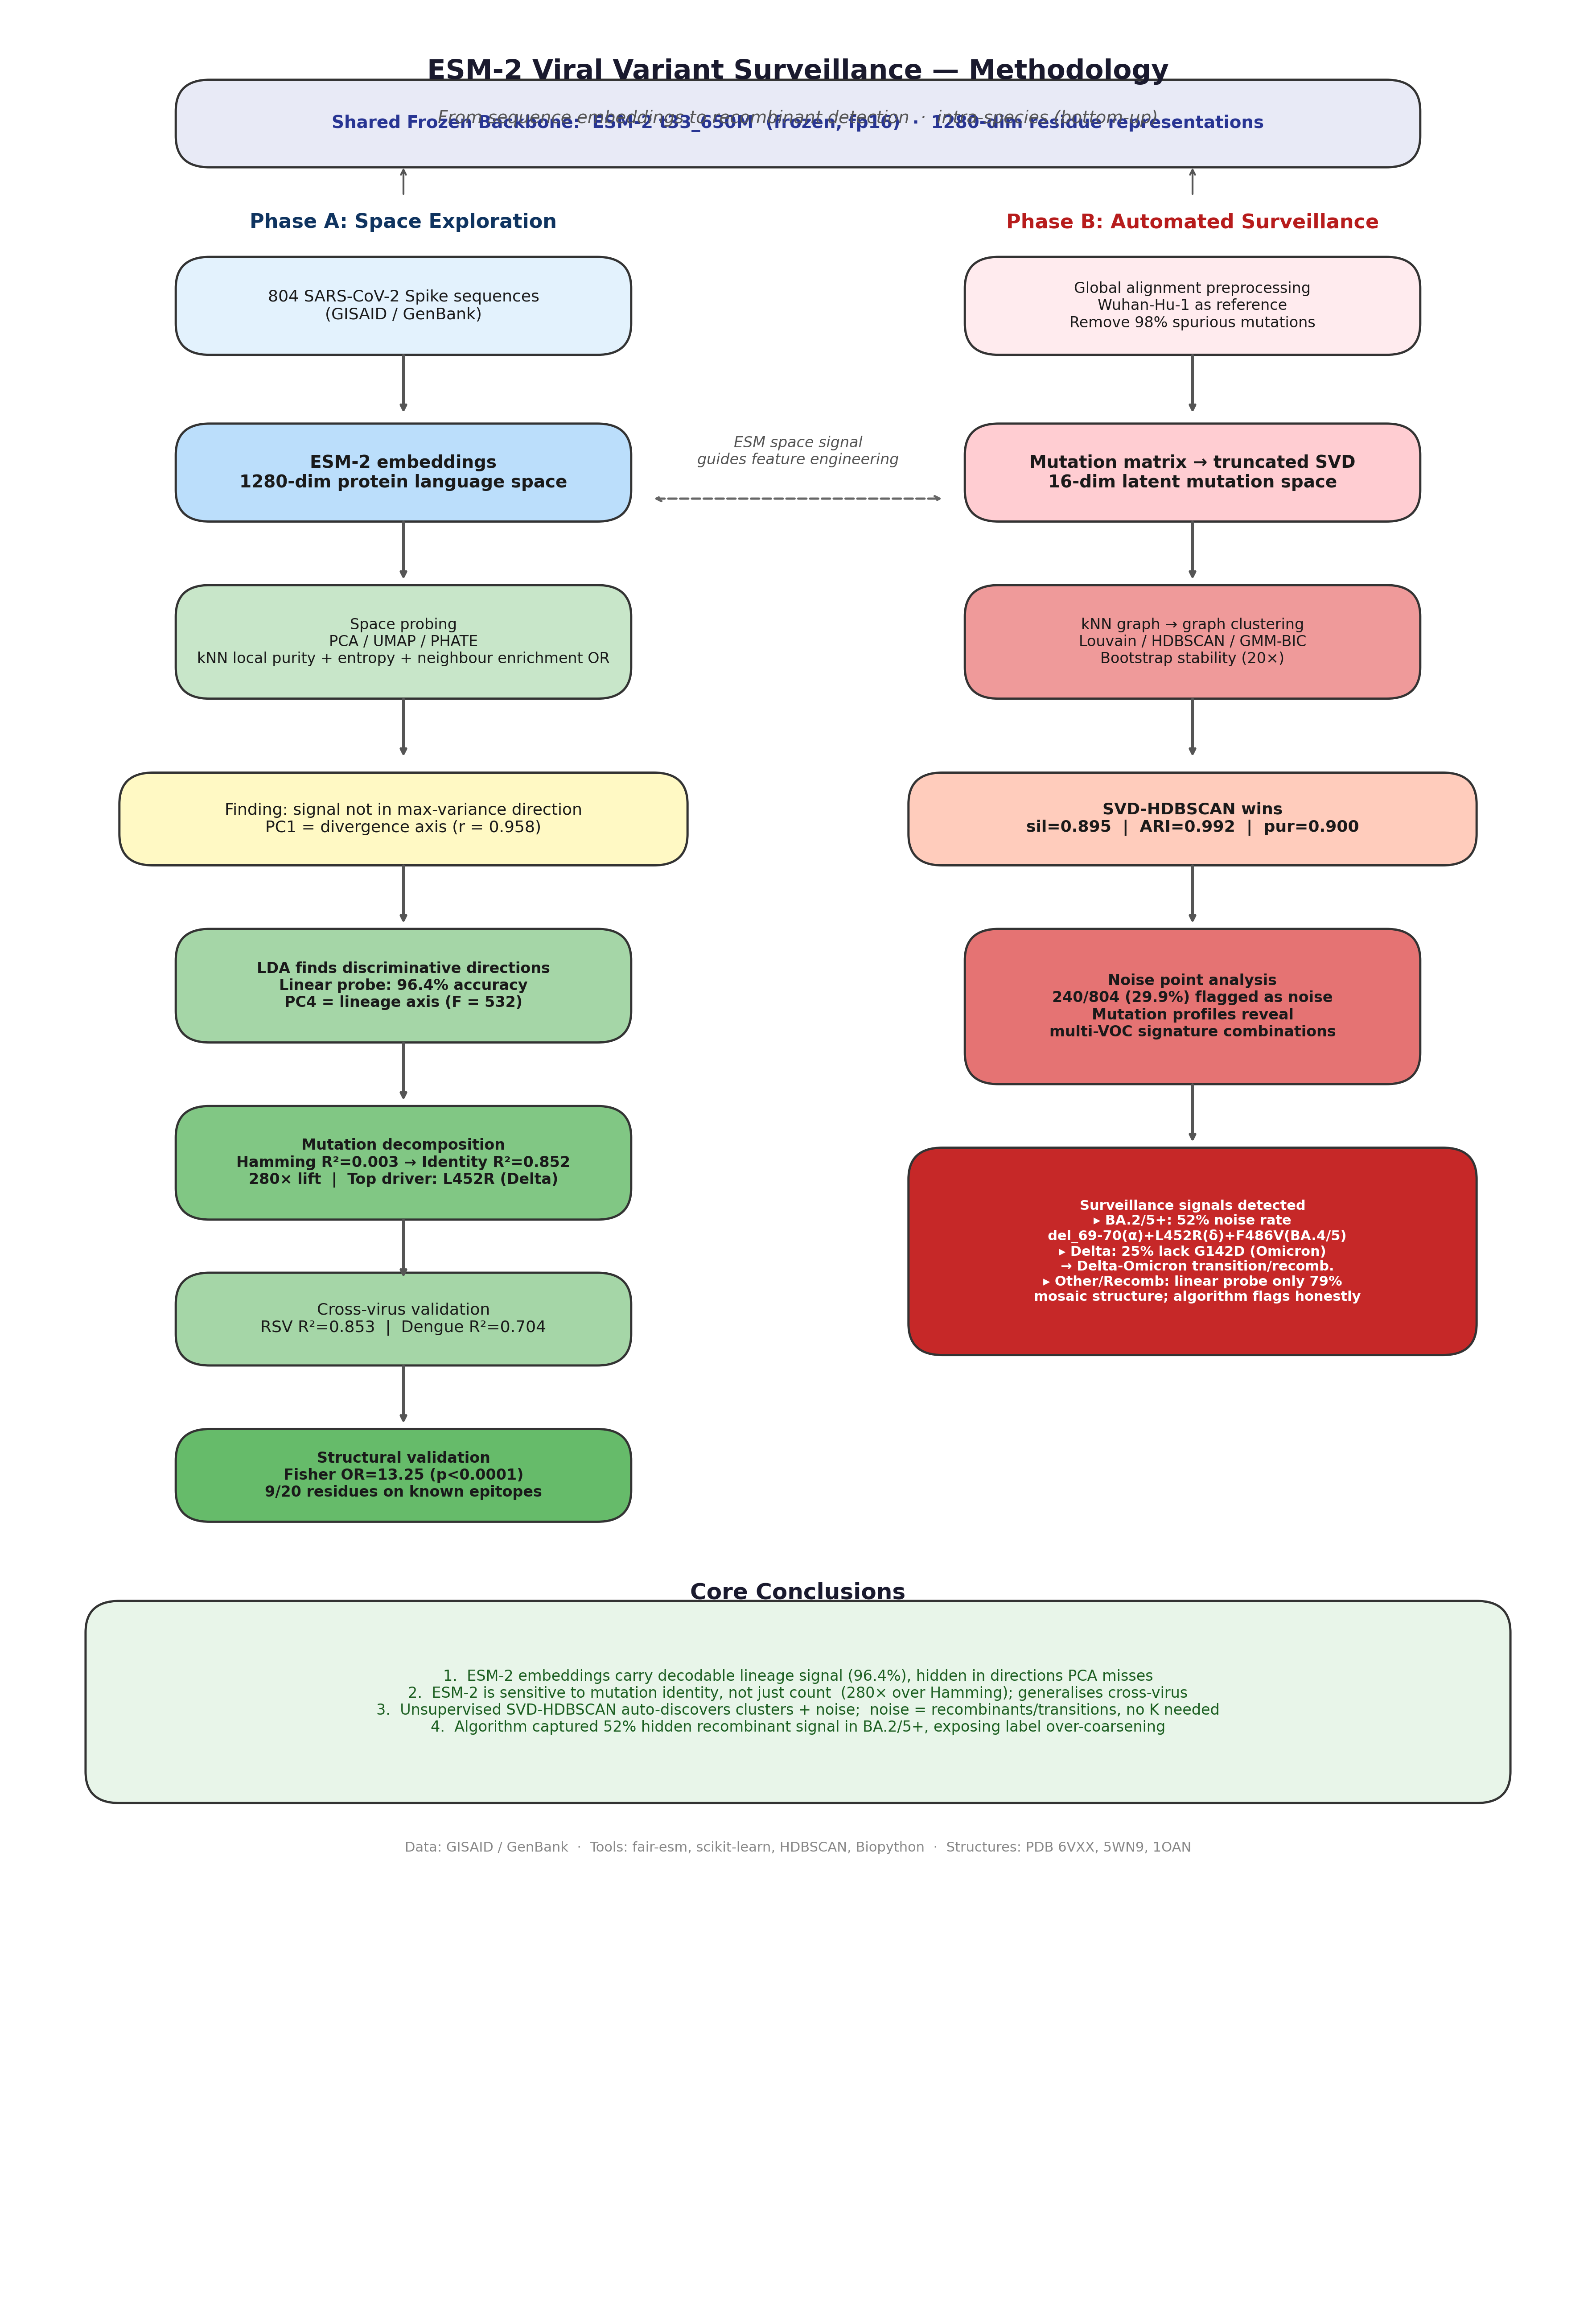
\includegraphics[width=\linewidth]{fig_methodology_unsupervised.png}
  \caption{Unsupervised surveillance pipeline. Phase A (left) diagnoses the ESM-2 representation space: PCA shows PC1 tracks Hamming distance while LDA recovers clean lineage separation, and sparse regression reveals mutation-identity R$^2\gg$ Hamming R$^2$. Phase B (right) applies truncated SVD ($k{=}16$) followed by HDBSCAN density clustering; noise points are retained as recombinant-candidate signals rather than discarded.}
  \label{fig:pipeline-unsup}
\end{figure}

\textbf{Data.} 804 SARS-CoV-2 Spike RBD sequences (GISAID + GenBank, 2020--2022) across six lineages: Ancestral, Alpha, Beta, Delta, Omicron BA.1, BA.2/5+. RSV F protein (n=410) and Dengue Envelope domain III (n=380) for cross-virus validation.

\textbf{Phase A: Representation diagnosis.} Frozen ESM-2-650M produces 1280-d mean-pooled embeddings. We project to 2D with PCA and LDA to diagnose the space, then run sparse linear regression to decompose ESM-2 pairwise distances into a Hamming component and a mutation-identity component. The ratio of identity R$^2$ to Hamming R$^2$ measures how much more ESM-2 cares about \textit{which} mutations occur versus \textit{how many}.

\textbf{Phase B: Clustering.} Truncated SVD ($k=16$ components) removes the top nuisance dimensions (dominated by sequence-length variance) without flattening the manifold. HDBSCAN ($\texttt{min\_cluster\_size}=15$, $\texttt{min\_samples}=5$) then operates on the SVD-compressed embeddings. We compare against: alignment + PCA + K-means (external baseline), ESM + direct K-means, ESM + HDBSCAN without SVD, and Autoencoder + GMM.

% ──────────────────────────────────────────────────────────────────────────────
\section{What We Found}
\label{sec:results}
% ──────────────────────────────────────────────────────────────────────────────

\subsection{Cross-species taxonomy}

\begin{table}[!htbp]
\caption{Per-rank accuracy on the held-out test set (5\% of genomes, stratified by Order).}
\label{tab:taxonomy}
\begin{center}
\begin{tabular}{lcccc}
\toprule
\textbf{Rank} & \textbf{Top-1} & \textbf{Top-5} & \textbf{Classes} & \textbf{Hier.\ Cons.} \\
\midrule
Kingdom & 99.71\% & 100.00\% & 2  & \\
Phylum  & 92.86\% & 99.71\%  & 9  & 94.86\% \\
Class   & 92.57\% & 99.14\%  & 15 & (all ranks) \\
Order   & 90.57\% & 98.86\%  & 41 & \\
\bottomrule
\end{tabular}
\end{center}
\end{table}

Table~\ref{tab:taxonomy} summarizes cross-species results; H1 passes on all metrics. The 94.86\% hierarchical consistency (332/350 predicted tuples exist in the training taxonomy) compares to near-zero for independent per-rank classifiers without the affiliate loss. The per-rank t-SNE plots in Figure~\ref{fig:tsne} make the degradation visible: Kingdom separation is nearly perfect, and structure degrades gracefully toward Order, mirroring the top-1 drop from 99.71\% to 90.57\%.

\begin{figure}[!htbp]
  \centering
  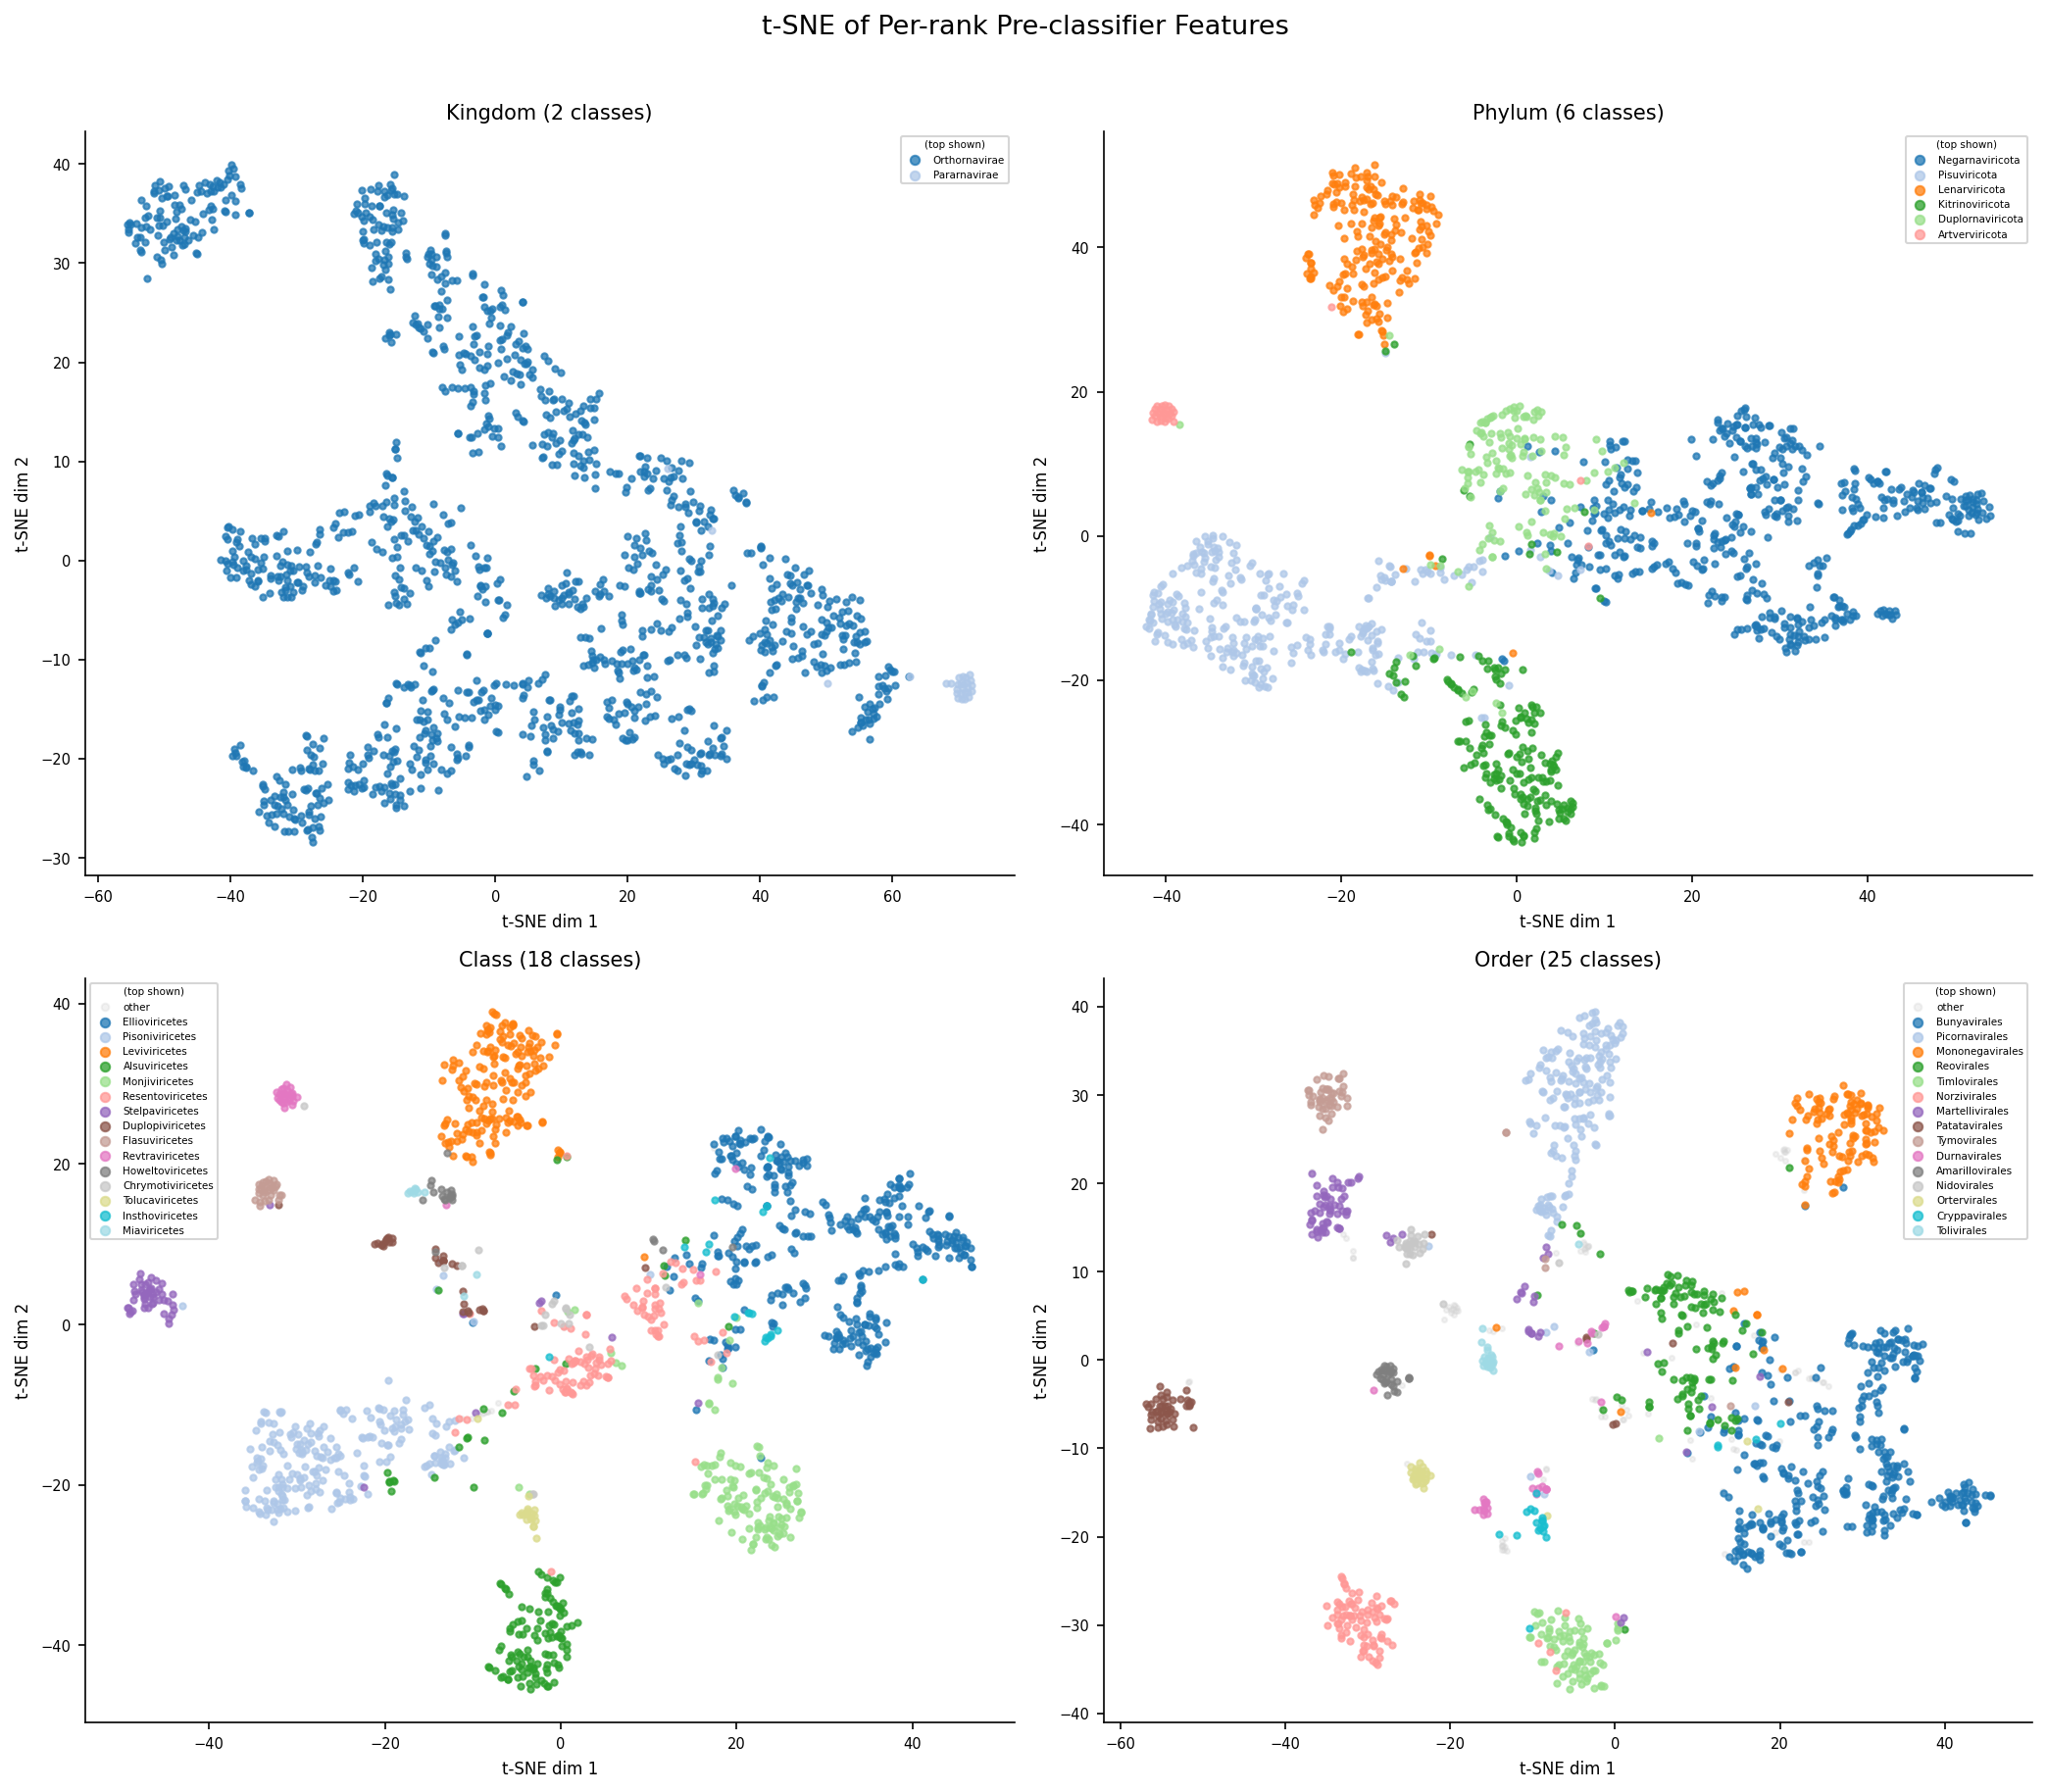
\includegraphics[width=0.82\linewidth]{fig_tsne_ranks.png}
  \caption{Per-rank t-SNE of cascade-decoder head features. Kingdom separates nearly perfectly; structure degrades gracefully toward Order, mirroring the top-1 drop from 99.71\% to 90.57\%.}
  \label{fig:tsne}
\end{figure}

\subsection{Mutation decomposition and layer probing}

\begin{figure}[!htbp]
  \centering
  \begin{minipage}[t]{0.49\linewidth}
    \centering
    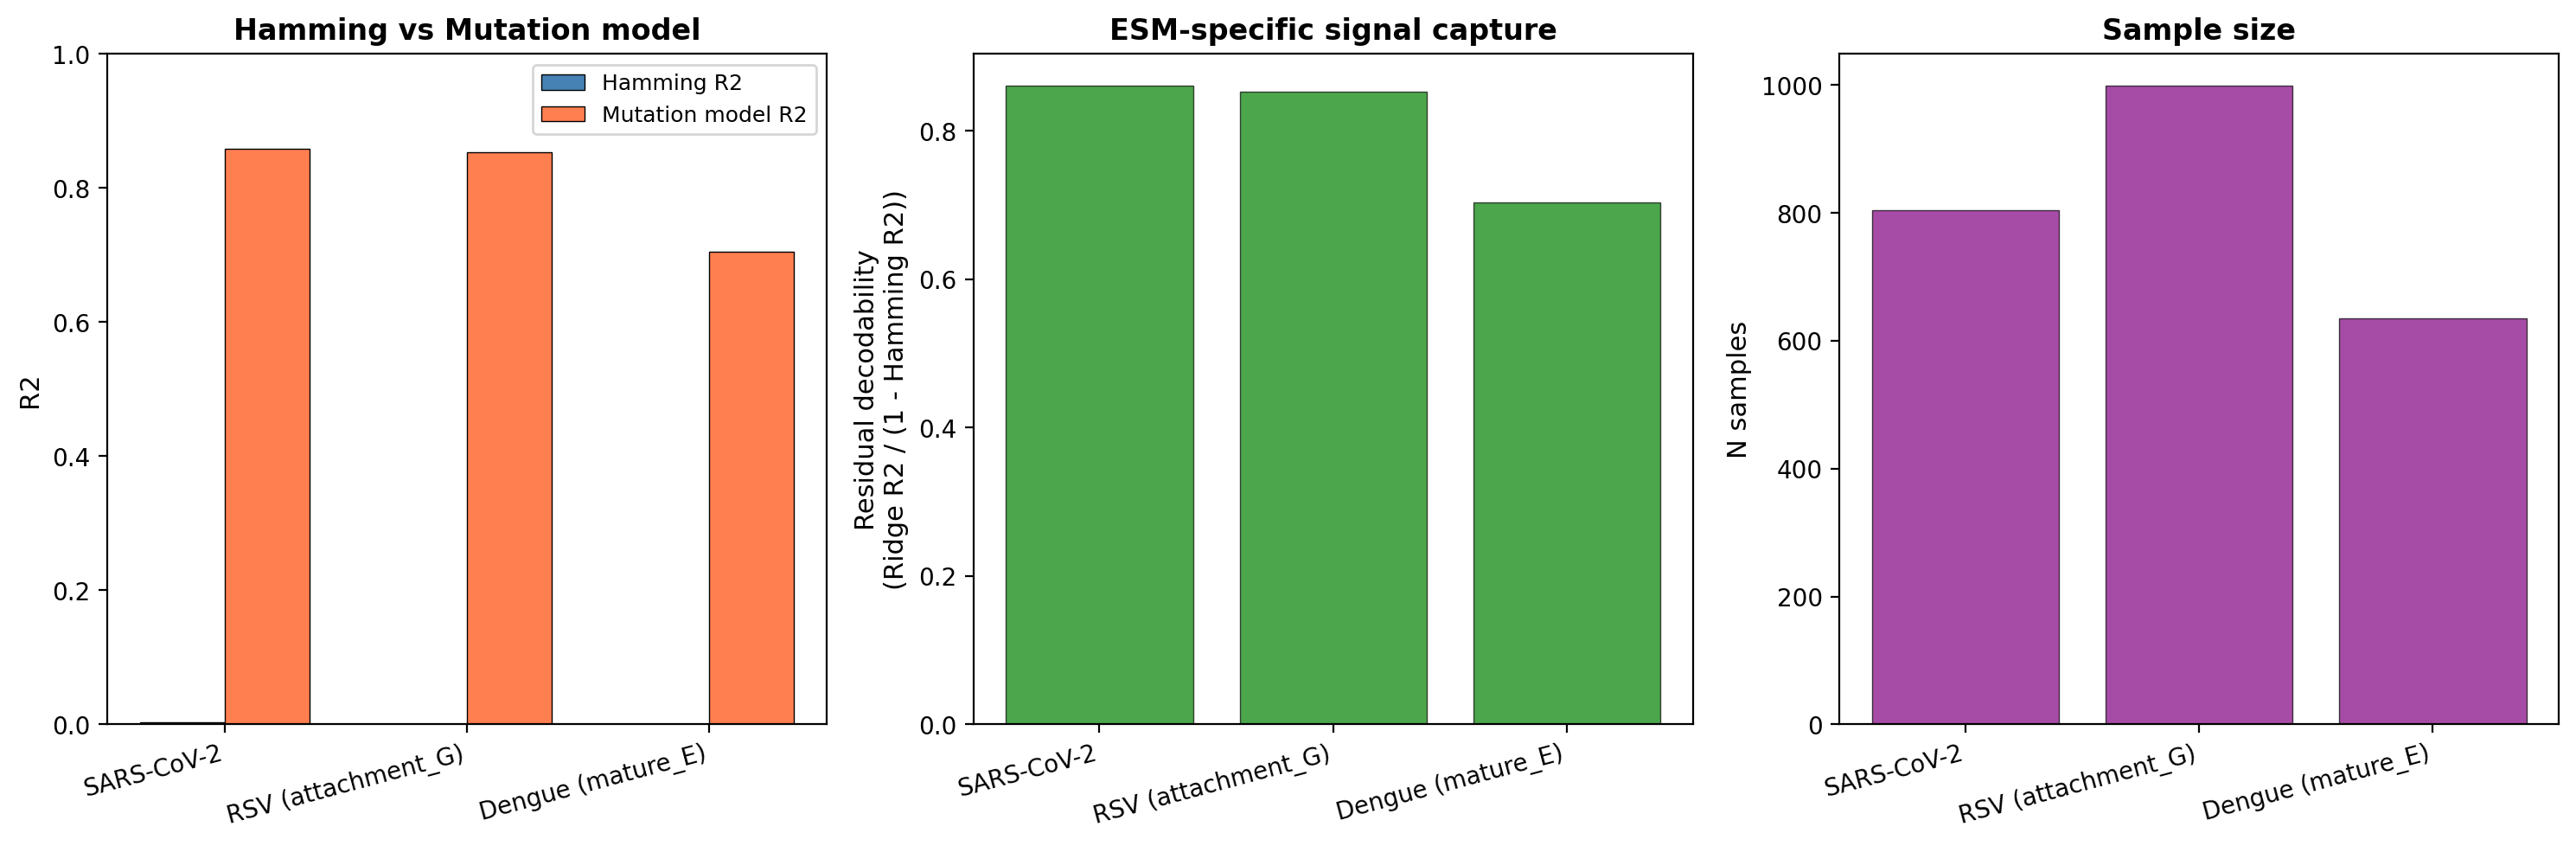
\includegraphics[width=\linewidth]{fig_mutation_decomp.png}
    \\[3pt]{\small (a) Mutation-identity vs.\ Hamming R$^2$ across three viruses.}
  \end{minipage}\hfill
  \begin{minipage}[t]{0.49\linewidth}
    \centering
    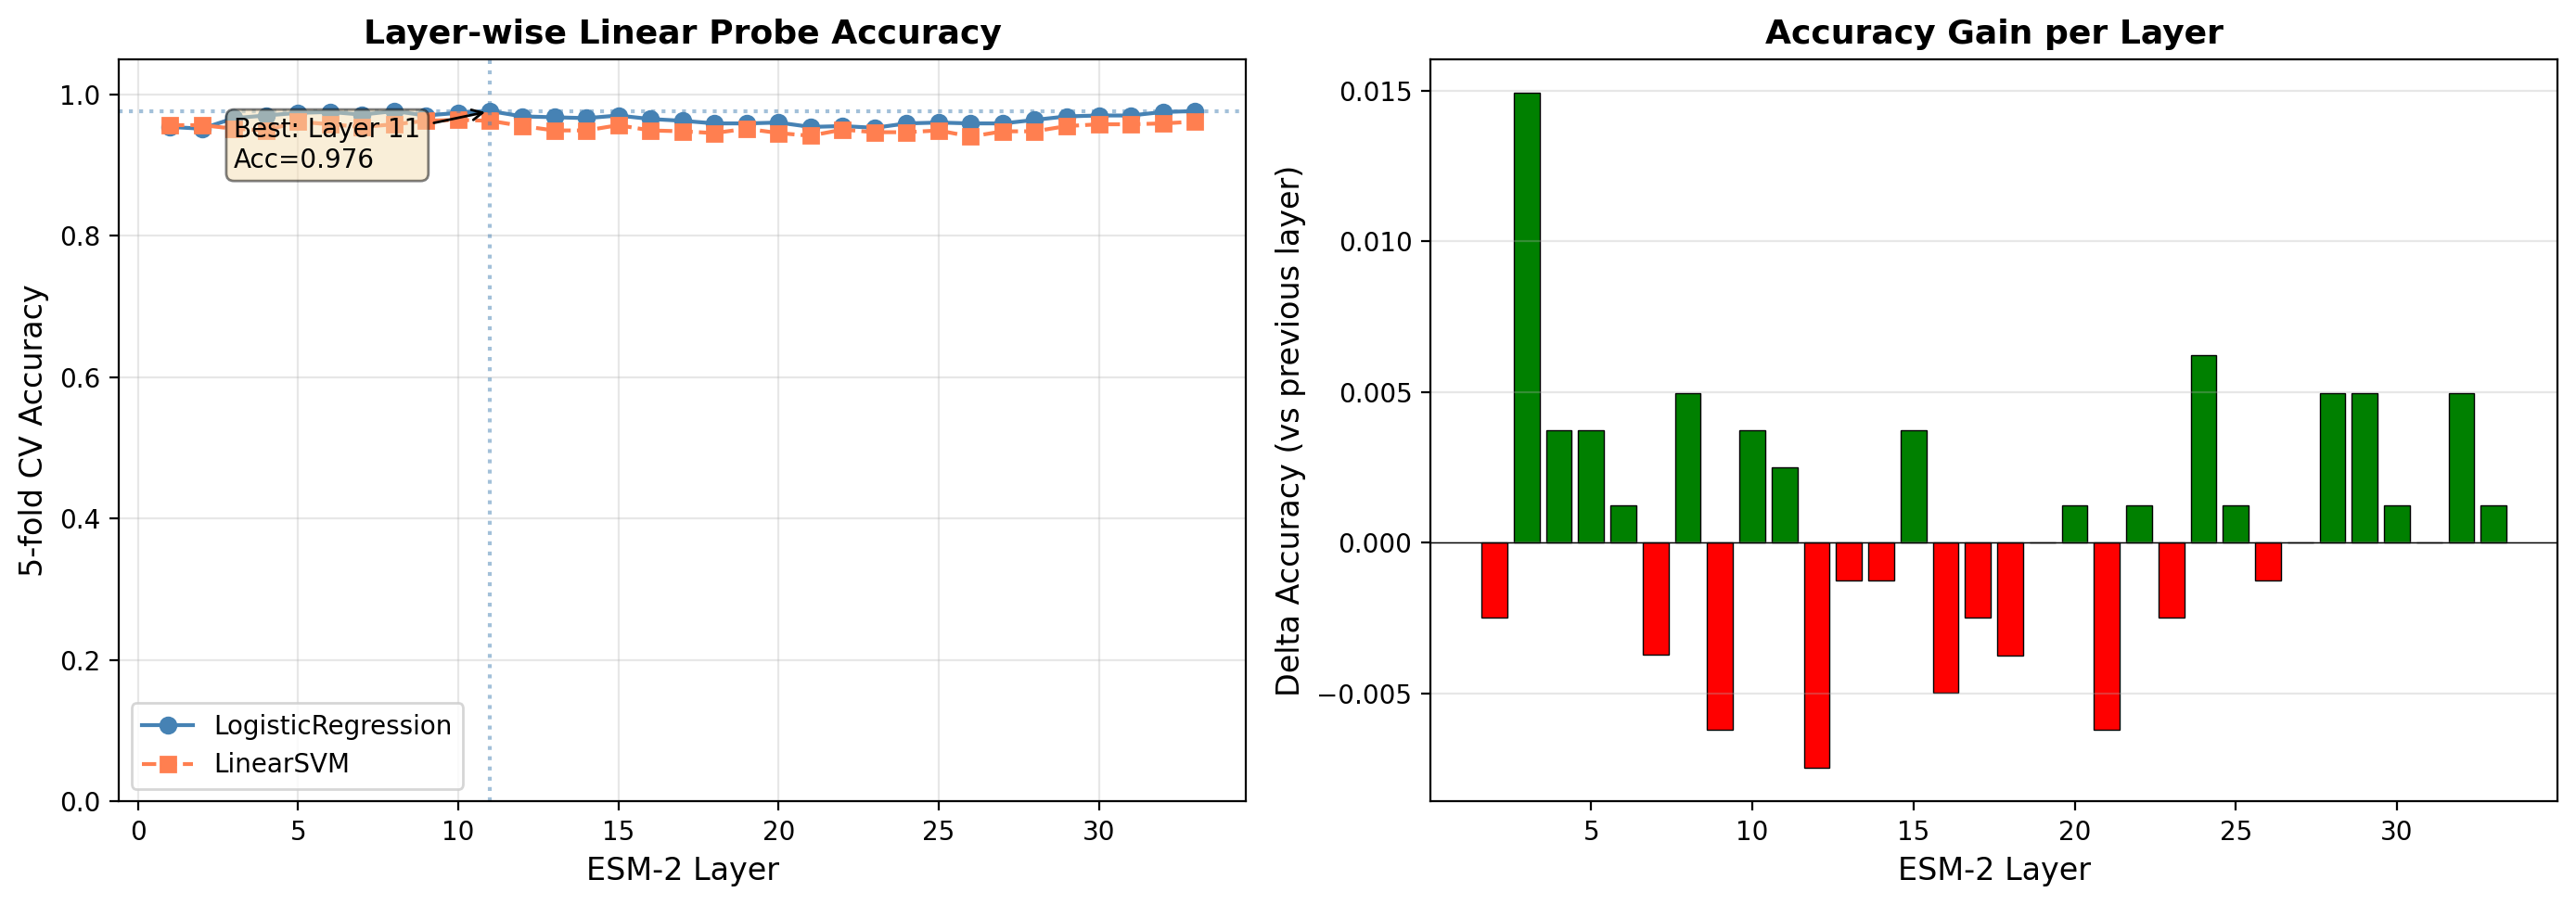
\includegraphics[width=\linewidth]{fig_layerwise_lda.png}
    \\[3pt]{\small (b) Layer-wise LDA probe accuracy (33 layers, ESM-2-650M).}
  \end{minipage}
  \caption{Mechanistic analysis. \textbf{(a)} Blue bars: Hamming R$^2$ ($\approx$0). Orange bars: mutation-identity R$^2$ (0.70--0.86). Gap is 280$\times$ (SARS-CoV-2), 850$\times$ (RSV), 704$\times$ (Dengue). ESM-2 encodes \emph{which} mutations occurred, not \emph{how many}. \textbf{(b)} Layer 1 already reaches 95.4\% LDA accuracy; the curve peaks at 97.6\% by Layer 8 and stays flat. Lineage-discriminative signal is present from the first transformer block, not a deep-emergence phenomenon.}
  \label{fig:mutdecomp}
  \label{fig:layerlda}
\end{figure}

Figure~\ref{fig:mutdecomp}(a) shows mutation-identity R$^2 = 0.852$ vs.\ Hamming R$^2 = 0.003$ for SARS-CoV-2 (280$\times$ gap), with RSV and Dengue producing nearly identical curves. ESM-2 encodes \emph{which} mutations happened, not \emph{how many}. H3a passes.

Figure~\ref{fig:mutdecomp}(b) shows Layer 1 LDA accuracy at 95.4\%, peaking at 97.6\% by Layer 8 and staying flat through Layer 33. Lineage discrimination is not a deep-emergence phenomenon; it appears in the first transformer block. H3b passes.

\subsection{Structural validation}

Integrated Gradients \citep{sundararajan2017ig} attribute importance to each residue. Figure~\ref{fig:structural} shows that top-20 positions by gradient magnitude fall inside known functional domains across all three viruses (Fisher exact OR = 13.25, $p{<}10^{-4}$ for SARS-CoV-2 NTD+RBD). H3c passes.

\begin{figure}[!htbp]
  \centering
  \begin{minipage}[t]{0.46\linewidth}
    \centering
    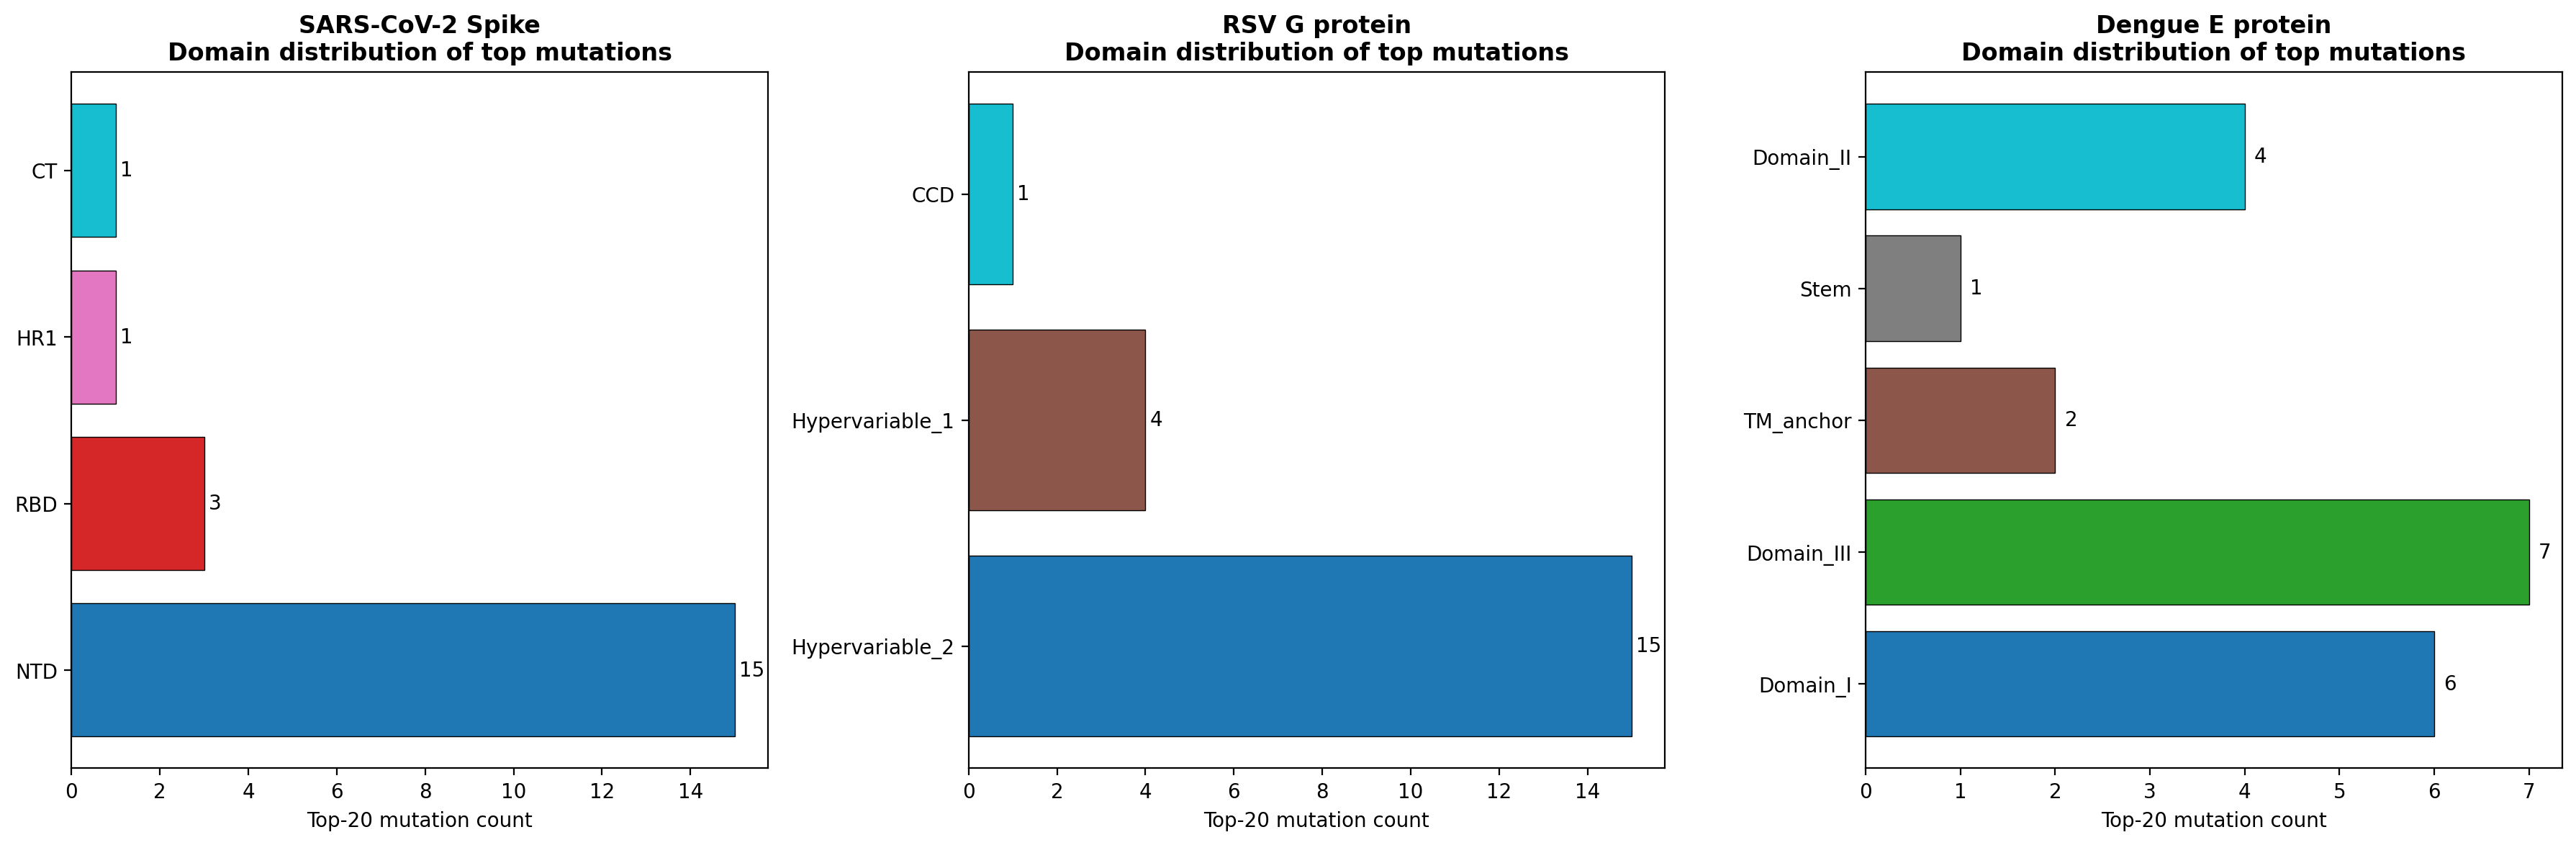
\includegraphics[width=\linewidth]{fig_domain_validation.png}
    \\[3pt]{\small (a) Domain enrichment: IG top-20 vs.\ functional domains.}
  \end{minipage}\hfill
  \begin{minipage}[t]{0.52\linewidth}
    \centering
    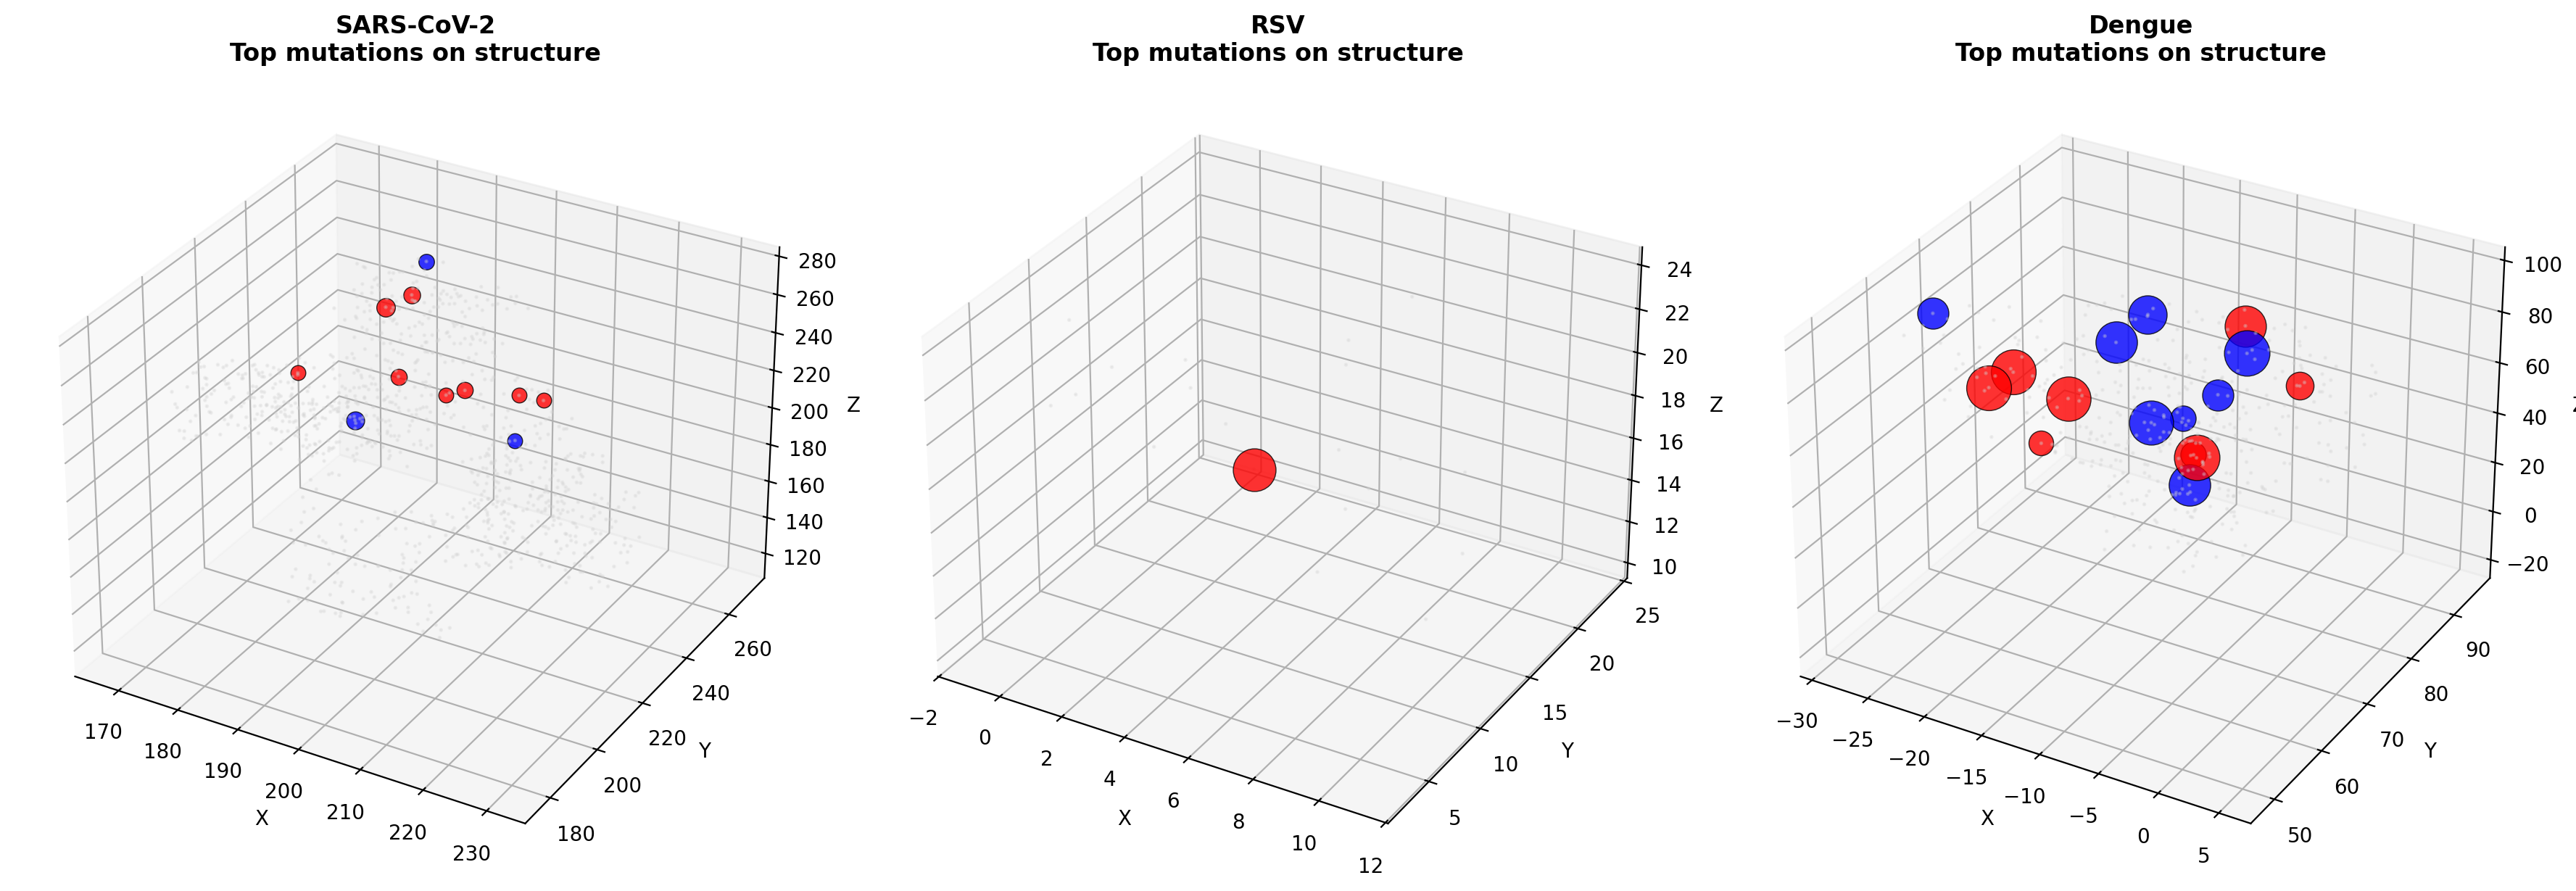
\includegraphics[width=\linewidth]{fig_3d_mapping.png}
    \\[3pt]{\small (b) IG-weighted residues mapped onto PDB 3D structures.}
  \end{minipage}
  \caption{Structural validation. (a) 18/20 top-attributed residues fall in NTD$+$RBD for SARS-CoV-2 (Fisher exact OR$=$13.25, $p{<}10^{-4}$); 19/20 in CCD for RSV. (b) Red spheres (positive attributions) cluster at receptor-binding interfaces---exactly where biologists would look.}
  \label{fig:structural}
\end{figure}

\subsection{Unsupervised variant clustering}

\begin{table}[!htbp]
\caption{Unsupervised clustering comparison on SARS-CoV-2 Spike (n = 804).}
\label{tab:clustering}
\begin{center}
\begin{tabular}{lcccc}
\toprule
\textbf{Method} & \textbf{Silhouette} & \textbf{Purity} & \textbf{ARI} & \textbf{Preset $k$} \\
\midrule
Alignment + PCA + K-means (external baseline\textsuperscript{†}) & 0.453 & --- & --- & Yes \\
ESM + K-means (Euclidean) & $\approx$0.30 & --- & --- & Yes \\
ESM + HDBSCAN & 0.697 & 0.75 & 0.99 & No \\
Autoencoder + GMM & 0.720 & 0.81 & 0.85 & Partial \\
\textbf{SVD + HDBSCAN (ours)} & \textbf{0.895} & \textbf{0.900} & \textbf{0.992} & \textbf{No} \\
\bottomrule
\end{tabular}
\end{center}
{\small \textsuperscript{†} Different dataset and preprocessing; shown as a representative upper bound for the alignment-based paradigm.}
\end{table}

Table~\ref{tab:clustering} shows that SVD-HDBSCAN dominates all baselines. Crucially, the alignment-based baseline appears clean (Figure~\ref{fig:baseline}) precisely because MSA has already forced sequences into a Euclidean-compatible subspace. ESM-2 embeddings do not have this property: global Euclidean distance conflates sequence-length variance, insertion/deletion patterns, and biological signal. Applying K-means directly to ESM-2 embeddings gives silhouette $\approx 0.30$, below the alignment baseline. The key insight is that \textit{local $k$-NN topology in ESM-2 space is stable and biologically meaningful} even though global Euclidean distance is not. SVD removes the top nuisance dimensions without flattening the manifold; HDBSCAN operates on local density, matching the geometry. H2 passes.

\begin{figure}[!htbp]
  \centering
  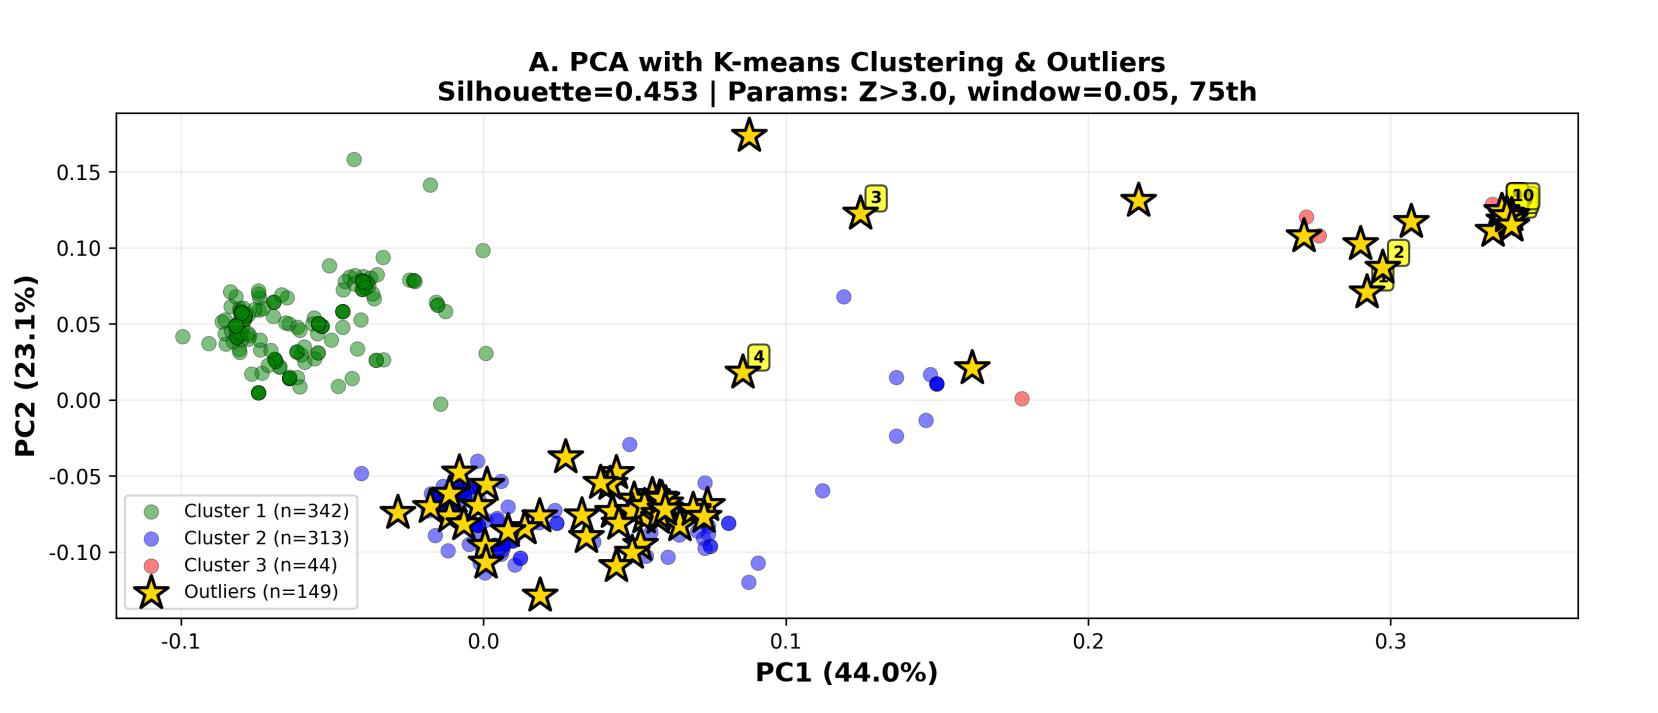
\includegraphics[width=0.72\linewidth]{fig_baseline_pca.png}
  \caption{External alignment + PCA + K-means baseline \citep{unsupervised2024dl}: silhouette = 0.453 on aligned SARS-CoV-2 Spike. Clean visual separation exists only because MSA pre-aligns sequences into a Euclidean-compatible subspace---a step unavailable for novel or highly divergent sequences.}
  \label{fig:baseline}
\end{figure}

\textbf{Recombinant detection.} HDBSCAN marks 240/804 sequences (29.9\%) as noise. This is not a failure: BA.2/5+ sequences have a 52.3\% noise rate (124/237), driven by simultaneous carriage of del69--70 (Alpha), L452R (Delta), and F486V (BA.4/5). The Pango BA.2/5+ label is too coarse; SVD-HDBSCAN splits it into at least three sub-clusters with distinct mutation co-occurrence patterns. Other lineages with high noise rates---Delta (25.2\%), BA.1 (25.2\%)---correspond to known transition zones. In short: what looks like clustering failure is phylogenetic signal.

% ──────────────────────────────────────────────────────────────────────────────
\section{Anything Interesting}
\label{sec:discussion}
% ──────────────────────────────────────────────────────────────────────────────

\textbf{Why deep learning.} The affiliate loss encodes parent-child constraints that a flat classifier cannot represent; the cascade decoder lets each rank condition on the parent's output. Together they produce a 4-order-of-magnitude jump in hierarchical consistency (0.02\% $\to$ 94.86\%). On the unsupervised side, Hamming distance explains near-zero variance in the ESM-2 directions that separate lineages---the representation is not recoverable from raw sequences. Deep learning provides the geometry; classical density methods exploit it.

\textbf{Manifold structure.} Lineage-discriminative signal appears in Layer 1 and stays flat through Layer 33---it is not a deep-emergence phenomenon. Combined with the failure of global Euclidean clustering and the success of HDBSCAN's local-density criterion, this places ESM-2 embeddings on a low-dimensional curved manifold. The right downstream tools are manifold-learning methods (Isomap, diffusion maps), not linear projection + Euclidean metrics. Formal characterization is the most natural extension of this work.

\textbf{Limitations and next steps.} Results use a single seed; error bars are pending. The surveillance dataset (n=804) is small. The most important open experiment is a time-extrapolation test: train on pre-2023 sequences and check whether 2024+ VOCs (XBB, JN.1, KP.*) appear as noise immediately. Future work: family-level held-out evaluation; formal manifold learning; scale to full GISAID ($10^5$--$10^6$ sequences) and $\geq$8 virus families.

% ──────────────────────────────────────────────────────────────────────────────
\subsubsection*{Acknowledgments}
Hardware: RTX 5060 Ti 16 GB, Windows 11, Python 3.11. Sequences from GISAID and GenBank. This project builds directly on \citet{passion2025virusproject}, which established the core ESM-based viral classification pipeline. AI assistance: Claude (Anthropic) assisted with code architecture, analysis scripting, and report writing. All experimental design, data interpretation, and scientific conclusions are the author's.

% ──────────────────────────────────────────────────────────────────────────────
\bibliography{esm_viral_refs}
\bibliographystyle{iclr2026_conference}

\end{document}
